\documentclass[10pt]{amsart}
\usepackage{style}

\title[Example]{Example: Functions are Not Differentiable at discontinuities}
\date{September 14, 2018}
\author{Blake Farman}
\address{Lafayette College}

\begin{document}
\maketitle

Consider the piecewise defined function
\[f(x) = \left\{\begin{array}{cc}x + 2 & \text{if}\ 0 \leq x,
\\x & \text{if}\ x < 0\end{array} \right.\]
which has a jump discontinuity at \(x = 0\):
\begin{center}
  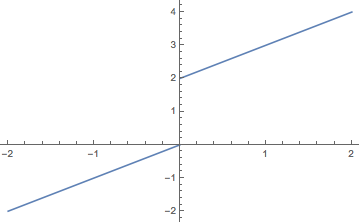
\includegraphics[scale=0.75]{function}
\end{center}

We saw in class today the following
\begin{thm}
  If \(f(x)\) is differentiable at \(x = a\), then \(f(x)\) is continuous at \(x = a\).
\end{thm}
As well as the equivalent 
\begin{thm}
  If \(f(x)\) is not continuous at \(x = a\), then \(f(x)\) is not differentiable at \(x = a\).
\end{thm}
The second formulation of the statement says that \(f(x)\) cannot be differentiable at \(x = 0\).
We can check this by explicitly computing the left and right hand limits of the definition of the derivative
\[\lim_{x \to 0} \frac{f(x) - f(0)}{x - 0} = \lim_{x \to 0} \frac{f(x) - 2}{x}.\]
The right-hand limit is simple to compute, and exactly what we expect:
\[\lim_{x \to 0^+} \frac{f(x) - 2}{x} = \lim_{x \to 0^+} \frac{x + 2 - 2}{x} = \lim_{x \to 0^+} \frac{x}{x} = \lim_{x \to 0^+} 1 = 1.\]

The left-hand limit
\[\lim_{x \to 0^-} \frac{f(x) - 2}{x} = \lim_{x \to 0^-} \frac{x - 2}{x}\]
requires slightly more care.
Since we know that
\[\lim_{x \to 0^-} x - 2 = 0 - 2 = -2\quad \text{and}\quad \lim_{x \to 0^-} x = 0\]
we can see that for very small negative numbers, the value of \((x - 2)/x\) will be large and positive (since both the numerator and denominator are negative), which is enough to conclude that
\[\lim_{x \to 0^-} \frac{x - 2}{x} = \infty.\]
One can see evidence for this, for example, by looking at the following table
\begin{center}
  \begin{tabular}{c|c}
    \(x\) & \(\displaystyle{\frac{x - 2}{x}}\)\\
    \hline\\
    \(\displaystyle{-10^{-1}}\) & \(21\)\\
    \(\displaystyle{-10^{-2}}\) & \(201\)\\
    \(\displaystyle{-10^{-3}}\) & \(2001\)\\
    \(\displaystyle{-10^{-4}}\) & \(20001\)
  \end{tabular}
\end{center}
or by plotting the function \((x-2)/x\)
\begin{center}
  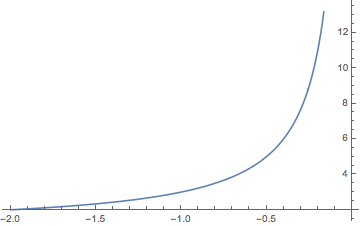
\includegraphics[scale=.75]{leftLimit}
\end{center}
In any case, this tells us that the left- and right-hand limits do not agree, so
\[\lim_{x \to 0} \frac{f(x) - f(0)}{x - 0} = \lim_{x \to 0} \frac{f(x) - 2}{x}\]
does not exist and thus the function \(f(x)\) is not differentiable at \(x = 0\).

\end{document}
